\documentclass{standalone}
\usepackage{tikz}
\usepackage{color}
\usetikzlibrary{positioning, shapes, arrows.meta, calc, decorations.pathreplacing}

\definecolor{myblue}{RGB}{82,126,171}
\definecolor{myred}{RGB}{168, 50, 50}

\tikzset{
  square/.style={draw,outer sep=5,inner sep=3,minimum size=10,line width=0, 
    very thick, draw=myblue, top color=white,bottom color=white},
  noborder/.style={draw,outer sep=0,inner sep=0,minimum size=20,line width=1, 
    draw=none, scale=1, anchor=west},
  blue/.style={draw,outer sep=35,inner sep=3,minimum size=20, line width=1, 
    very thick, draw=none, top color=myblue, bottom color=myblue, scale=1.25}
}

\begin{document}

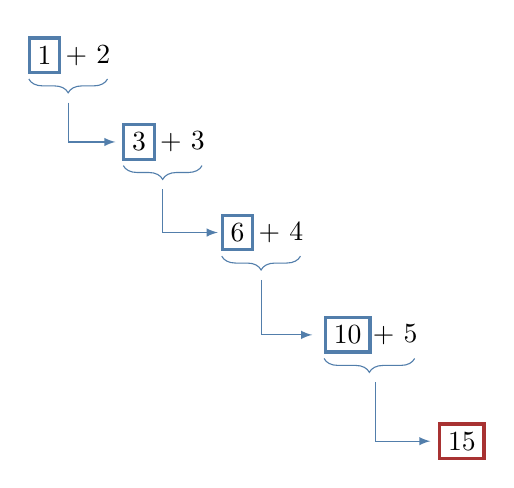
\begin{tikzpicture}[>={Latex[width=2mm,length=2mm]}]

\node [square] at (-1.25,1.7) {$1$};
\node [noborder] at (-1.05,1.7) {+ 2};
\draw[decorate,color=myblue,decoration={brace,amplitude=5pt}] (-0.45,1.4) -- (-1.45,1.4);
\draw[-latex,color=myblue] (-0.95,1.1) |- (-0.35,0.6);

\node [square] at (-0.05,0.6) {$3$};
\node [noborder] at (0.15,0.6) {+ 3};
\draw[decorate,color=myblue,decoration={brace,amplitude=5pt}] (0.75,0.3) -- (-0.25,0.3);
\draw[-latex,color=myblue] (0.25,0) |- (0.95,-0.55);

\node [square] at (1.2,-0.55) {$6$};
\node [noborder] at (1.4,-0.55) {+ 4};
\draw[decorate,color=myblue,decoration={brace,amplitude=5pt}] (2,-0.85) -- (1,-0.85);
\draw[-latex,color=myblue] (1.5,-1.15) |- (2.15,-1.85);

\node [square] at (2.6,-1.85) {$10$};
\node [noborder] at (2.85,-1.85) {+ 5};
\draw[decorate,color=myblue,decoration={brace,amplitude=5pt}] (3.45,-2.15) -- (2.3,-2.15);
\draw[-latex, color=myblue] (2.95,-2.45) |- (3.65,-3.2);

\node [square, draw=myred] at (4.05,-3.2) {$15$};

\end{tikzpicture}

\end{document}
